	
\documentclass[a4paper,12pt]{article} 
    \usepackage{amsmath, amssymb}
    \usepackage{kotex}
    \usepackage{graphicx}
    \usepackage[figuresright]{rotating} 
    
    \begin{document} 
    
    \title{과제6 보고서}
    \author{B211103 변준석}
    \date{2017년 10월}
    \maketitle

    \newpage
    \section{개요}
    이번 과제의 메인 프로그램인 \textsl{hw6.cpp} 에서는 스택 자료구조를 이용하여 수식의 중위표기를 후위표기로 변환하는 프로그램을 구현하였다.
    
    \section{문제 해결 방안}
    중위표기식을 \textsl{Expression}구조체에 저장, \textsl{Token}구조체로 피연산자, 연산자, 괄호를 단위크기로 저장/운반하였다.  \textsl{Token}의 스택을 구현하여 후위표기식으로 변환하는데 필요한 연산자의 위치 변환에 사용하였다.
    
    \section{\textsl{최종 출력}}
    \newpage
    \begin{figure}[t]\vspace*{4pt} 
    \centerline{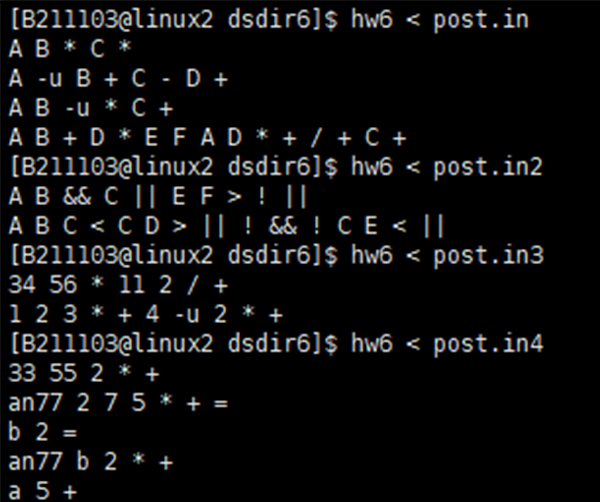
\includegraphics[width=1.0\columnwidth]{result}} 
    \caption{입력 파일과 실행했을 때의 결과}\vspace*{-6pt} 
    \label{figure:result} 
    \end{figure} 
    
    
    \section{hw6의 간단한 설명}
    모든 기능들이 정상작동함을 알 수 있다. 알파벳으로 이루어진 피연산자, 숫자로 이루어진 피연산자, 1글자 연산자, 2글자 연산자, 괄호 모두 다르게 처리해주어야하며, \textsl{Token}의 스택에 쌓이는 우선순위와 스택을 나가는 우선순위를 따로 지정해주어야 한다.

    
    \newpage
    \begin{figure}[t]\vspace*{4pt} 
    \centerline{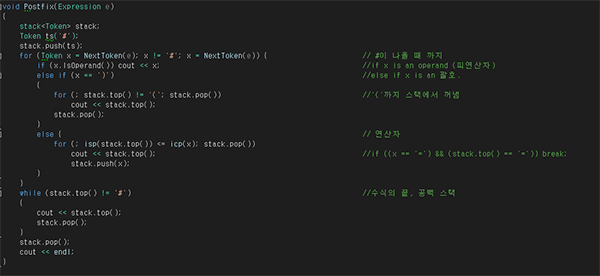
\includegraphics[width=1.0\columnwidth]{f1}} 
    \caption{post.cpp의 Postfix 함수}\vspace*{-6pt} 
    \label{figure:f1} 
    \end{figure} 
    
    \begin{figure}[t]\vspace*{4pt} 
    \centerline{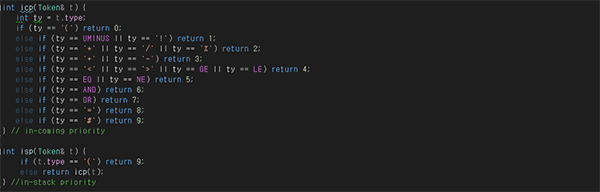
\includegraphics[width=1.0\columnwidth]{f2}} 
    \caption{post.cpp의 icp / isp 함수}\vspace*{-6pt} 
    \label{figure:f2} 
    \end{figure} 
    
    \newpage
    \begin{figure}[t]\vspace*{4pt} 
    \centerline{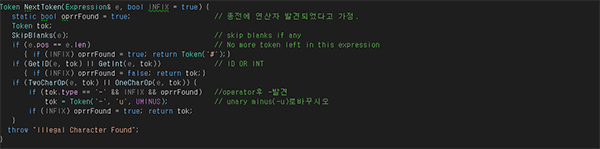
\includegraphics[width=1.0\columnwidth]{f3}} 
    \caption{post.cpp의 NextToken 함수}\vspace*{-6pt} 
    \label{figure:f3} 
    \end{figure} 
    
    \begin{figure}[t]\vspace*{4pt} 
    \centerline{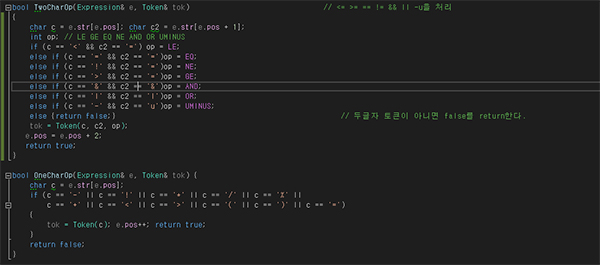
\includegraphics[width=1.0\columnwidth]{f4}} 
    \caption{post.cpp의 TwoCharOp, OneCharOp 함수}\vspace*{-6pt} 
    \label{figure:f4} 
    \end{figure} 
    
    \begin{figure}[t]\vspace*{4pt} 
        \centerline{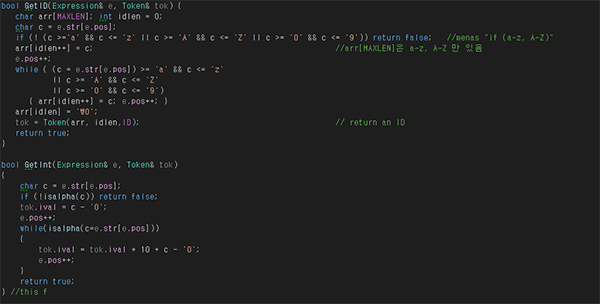
\includegraphics[width=1.0\columnwidth]{f5}} 
        \caption{post.cpp의 GetID, GetInt 함수}\vspace*{-6pt} 
        \label{figure:f5} 
        \end{figure} 
        
    \end{document} 